\documentclass{article}  
\title{algorithm}
\usepackage{CJKutf8}
\usepackage{listings}
\usepackage{amsmath}
\usepackage{amsfonts}
\usepackage{mathtools,amssymb}
\usepackage{graphicx}
\usepackage{mathrsfs}  
\begin{document}

\begin{CJK}{UTF8}{gbsn} 
	匹配和转录的算法通常遵循所提供的模式或模板的递归结构。 匹配使用模式p来实施与tokens tree序列s的等同性,同时将变量x添加到模式环境Θ中。 Transcribe使用模板t来生成新的语法s,方法是用基于Θ的替换替换所有的自由模式变量x。
\end{CJK}	

\begin{equation}
	match : p * s * \theta \rightarrow (\theta, s);\\
    transcribe : t * \theta \rightarrow s
\end{equation}

\begin{CJK}{UTF8}{gbsn}
	下面给出一个代码,显示了一个简单的匹配和转录的例子,作为宏扩展的一部分。
	
\end{CJK}
$
\\
expand_{\sum} \; ( unless \cdot (success) \quad fail();) \\
\hookrightarrow  match (x \cdot y, (success)fail(); \qquad  \varnothing )\\
\rightarrow match (y, fail() ;,  \qquad[x\mapsto (success)]) \\
\rightarrow match (\epsilon ,;,\qquad[x\mapsto (success),y\mapsto fail()])\\
\hookrightarrow transcribe ( if ( ! x) \cdot y,\qquad[x\mapsto (success),y\mapsto fail()])\\
\rightarrow if (!(success))\quad fail();\\
\\
$

\begin{CJK}{UTF8}{gbsn} 
	完整的算法则如下所示。
\end{CJK}

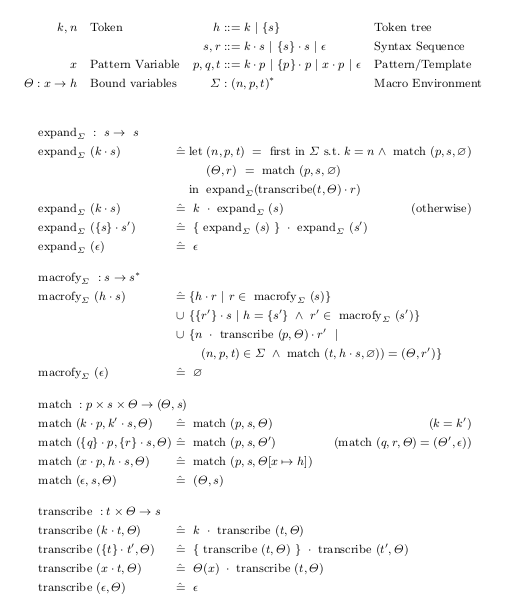
\includegraphics[scale = 0.9]{algorithm.png}

\begin{CJK}{UTF8}{gbsn}
	这个算法看起来比较复杂,这里大致讲一下思路:
	这里给出一个例子:	
\end{CJK}

\begin{lstlisting}
macro foo {
  {
    (x=>$e:expr)
  } => {
    console.log('got a ', $e)
  }
}
foo(x=>3) 
// => console.log("got a ", 3)
\end{lstlisting}


\begin{CJK}{UTF8}{gbsn}
在这里,实际上sweet.js做了Reader和Expander的工作:
1.lexer 把源码token化, 得到token序列
2.Reader把token变成token树
3.变term树
4.Expander按照定义的macro匹配扩展token树, 再parse成AST

这种转换方法太过暴力和简单,这里只能做一些非常简单的形式上的一一变化,如果想要元编程,那么太复杂不能变数据,只能变AST来操作复杂的语法树:
\end{CJK}

\begin{lstlisting}
  macro m {
    case {ctx (x=>$x)} => {
      console.log('haha iam javascript')
      return #{
       console.log($x) 
      }
    }
  }
  m(100) 
//=> haha iam javascript (to console)
//=> console.log(100)
\end{lstlisting}

\begin{CJK}{UTF8}{gbsn}
在这里,实际上sweet.js做了Reader和Expander的工作:
1.lexer 把源码token化, 得到token序列
2.Reader把token变成token树
3.变term树
4.Expander按照定义的macro匹配扩展token树, 再parse成AST

这种转换方法太过暴力和简单,这里只能做一些非常简单的形式上的一一变化,如果想要元编程,那么太复杂不能变数据,只能变AST来操作复杂的语法树:
\end{CJK}

\begin{CJK}{UTF8}{gbsn}
多了一个参数 ctx,匹配用到m时的那个m
接下来都一样, 直到星号后面的内容
这里面的语法变成语法树, 当然语法树结构是数组, 每个元素还是一个token树.比如console.log(3)大概是这种结构
\end{CJK}
\begin{lstlisting}
[
    {token: {value: 'console'}}
    {token: {value: '.'}},
    {token: {value: 'log'}},
    {token: {value: '()'},
     inner:[
         {token: {value: 3}}
     ]}
]
\end{lstlisting}

\begin{CJK}{UTF8}{gbsn}
最重要的, 现在里面可以写正常js了, 意味着你可以用js编程各种语法,然后拼到token树中
\end{CJK}

\end{document}